% fig-5.tex — standalone figure. One tikzpicture only. Preamble fixed.
\documentclass[border=3pt]{standalone}
\usepackage{tikz}
\usetikzlibrary{arrows.meta,decorations.markings,angles,quotes,patterns,calc}
\definecolor{seccolor}{RGB}{30,90,140}
\definecolor{rulecolor}{RGB}{205,150,35}
\definecolor{accent}{RGB}{180,60,40}
\definecolor{accent2}{RGB}{40,120,90}
\definecolor{lightfill}{RGB}{232,240,247}
\begin{document}
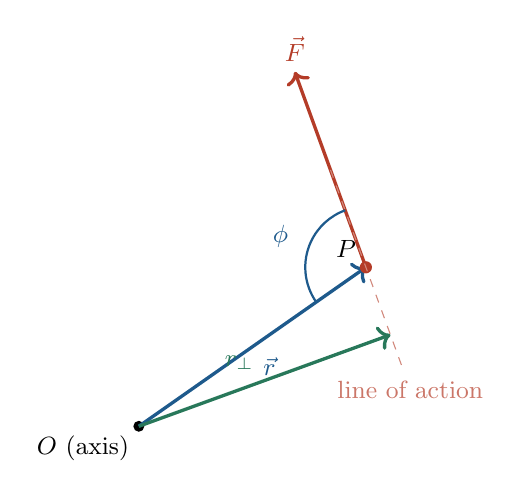
\begin{tikzpicture}[scale=1.1]
  \fill (0,0) circle (1.8pt);
  \node[below left] at (0,0) {\small $O$ (axis)};
  \coordinate (P) at (35:3.2);
  \draw[->,seccolor,very thick] (0,0)--(P) node[midway,below right]{\small $\vec{r}$};
  \fill[accent] (P) circle (2pt);
  \node[above left] at (P) {\small $P$};
  \coordinate (Fdir) at ($(P)+(110:2.4)$);
  \draw[->,accent,very thick] (P)--(Fdir) node[above]{\small $\vec{F}$};
  \draw[accent!60,dashed] ($(P)!-1.2cm!(Fdir)$)--($(P)!1.2cm!(Fdir)$);
  \node[accent!70] at ($(P)!-1.5cm!(Fdir)$) {\small line of action};
  \coordinate (Q) at ($(P)!(0,0)!(Fdir)$);
  \draw[->,accent2,very thick] (0,0)--(Q) node[midway,above left]{\small $r_\perp$};
  \draw[seccolor,thick] (P)+(215:0.7) arc (215:110:0.7);
  \node[seccolor] at ($(P)+(160:1.05)$) {\small $\phi$};
\end{tikzpicture}
\end{document}
